\subsection*{Results and Discussion}
As discussed in the previous section, we first find the optimal rank $R$ for the model.
We did this by fitting 20 models with different random initializations for $R \in \{1,2,3,4,5\}$, and computing the loss and RelFit for the best model for each $R$.
The results are shown in Table \ref{tab:rank_choice}.
Note that the loss is relative to the loss of the best model with rank $R=1$.

\begin{table}[H]
    \centering
    \begin{tabular}{|c|c|c|}
    \hline
    $R$ & Loss & RelFit \\
    \hline
    1 & 1 & 77.589 \\
    \hline
    2 & 0.0975 & 96.497 \\
    \hline
    3 & 0.0065 & 98.891 \\
    \hline
    4 & 0.0045 & 98.936 \\
    \hline
    5 & 0.0028 & 98.967 \\
    \hline
    \end{tabular}
    \caption{Loss relative to loss with rank $R=1$ and RelFit for $R\in \{1,2,3,4,5\}$ for best model of 20 runs for each $R$.}
    \label{tab:rank_choice}
\end{table}

From Table \ref{tab:rank_choice}, we see that the loss is decreasing by a factor greater than $ 10$ for each $R$ until $R=3$, after which it decreases by a factor less than $ 2$.
Furthermore, the relative fit increases substantially from $R=1$ to $R=2$ and $R=2$ to $R=3$, after which the growth is significantly slower.
Hence $R=3$ seems like a good choice of rank, and we use this for further analysis.
Figure \ref{fig:plot_factors} confirms this choice, as we see that the factors for $R=3$ seems to represents three different chemicals, while for $R=4$, the red and green factor seems to both represent the same chemicals, as they are more or less identical in the emission and excitation modes.

Next, we ran the model with $R = 3$ as rank 20 times, in this case saving all the obtained models.
Comparing the models, we saw that all models reached the exact same loss.
Furthermore, they all achieved an FMS of 1 when compared to the first model using the \texttt{score} function.
That is, all models ended with the exact same fit regardless of initialization, which demonstrates that the uniqueness of the factors revealed by the CP decomposition.
As a sanity check, we did the same analysis for $R=4$, where we only had 17 out of the 20 models within 2\% of the loss, and most models achieved an FMS of less than $0.95$ when compared to the best model.
This finding confirms that the exact matches discovered for rank $R=3$ is not due to some error in our method of comparison.

\begin{figure}[H]
    \centering
    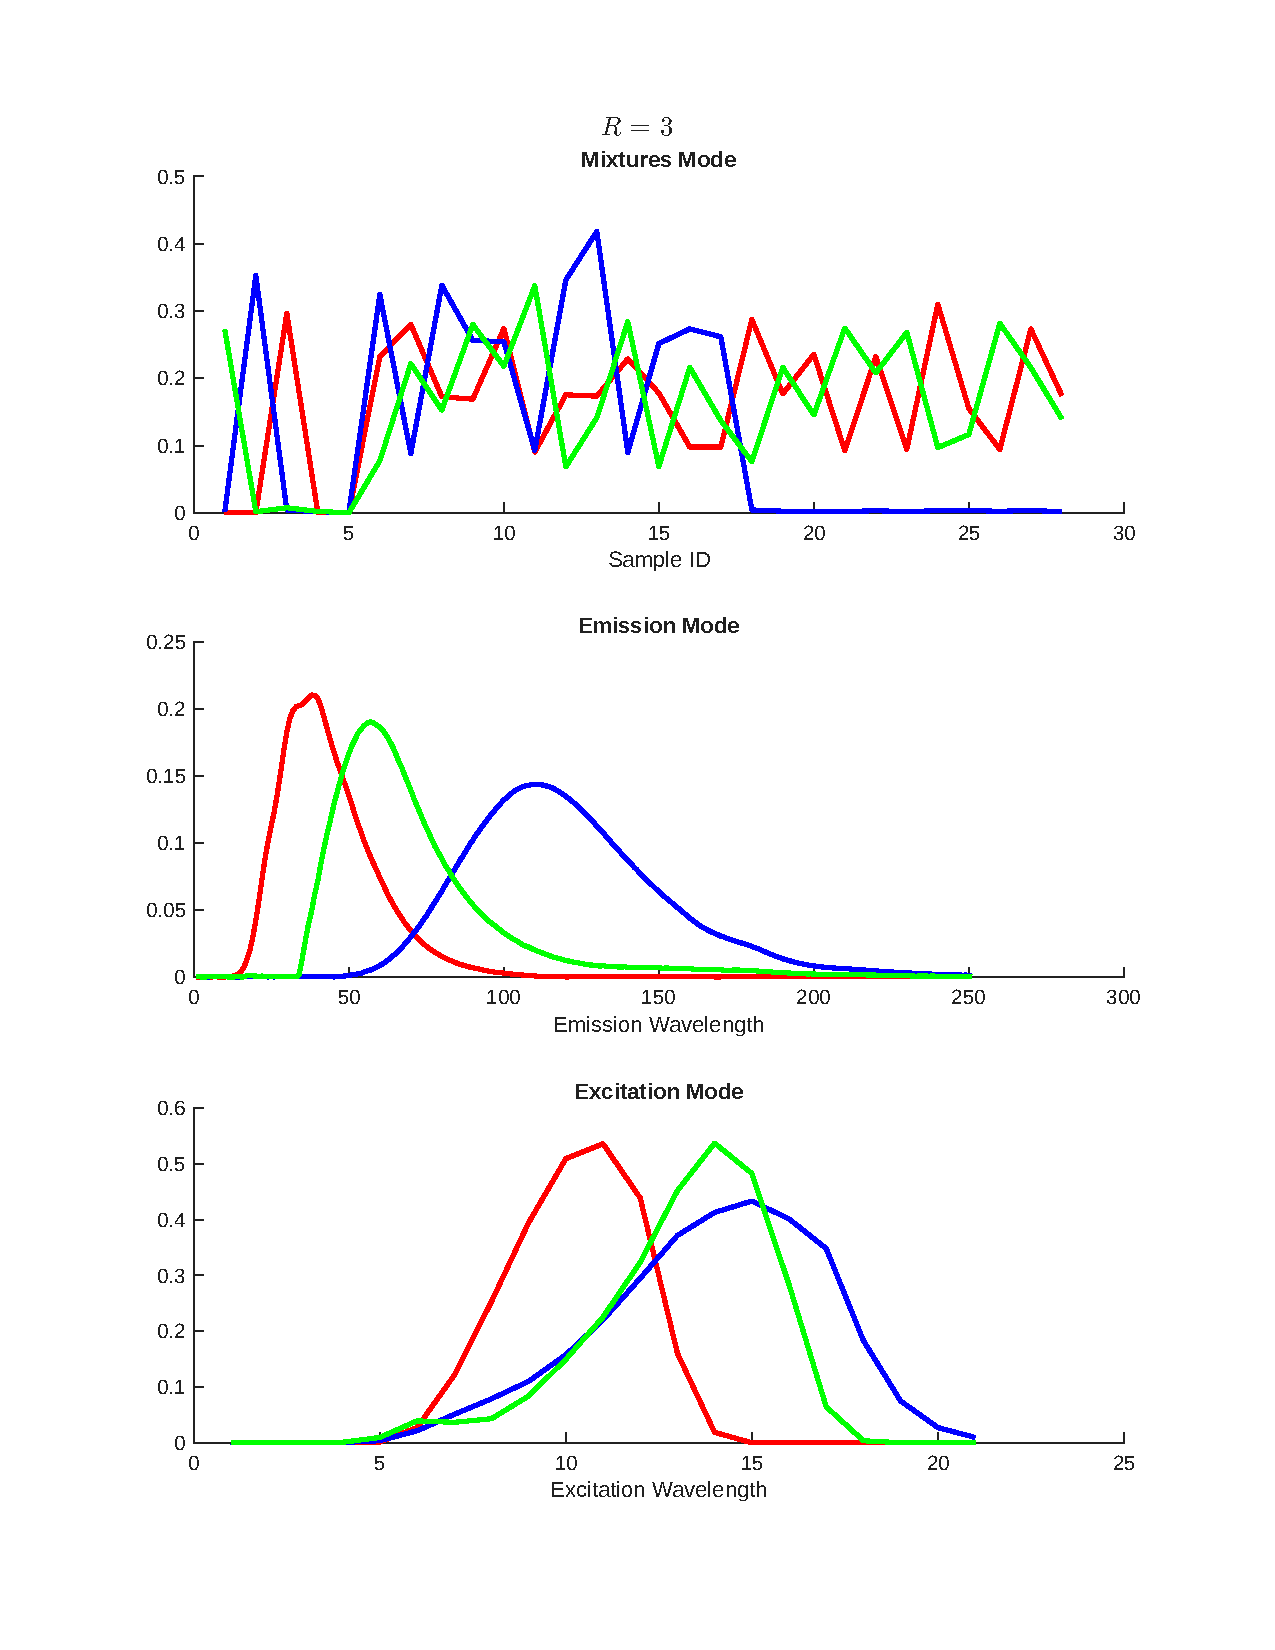
\includegraphics[trim = 2cm 2.5cm 2cm 1.9cm, clip, width=0.46\linewidth]{figures/factors_rank3.pdf}
    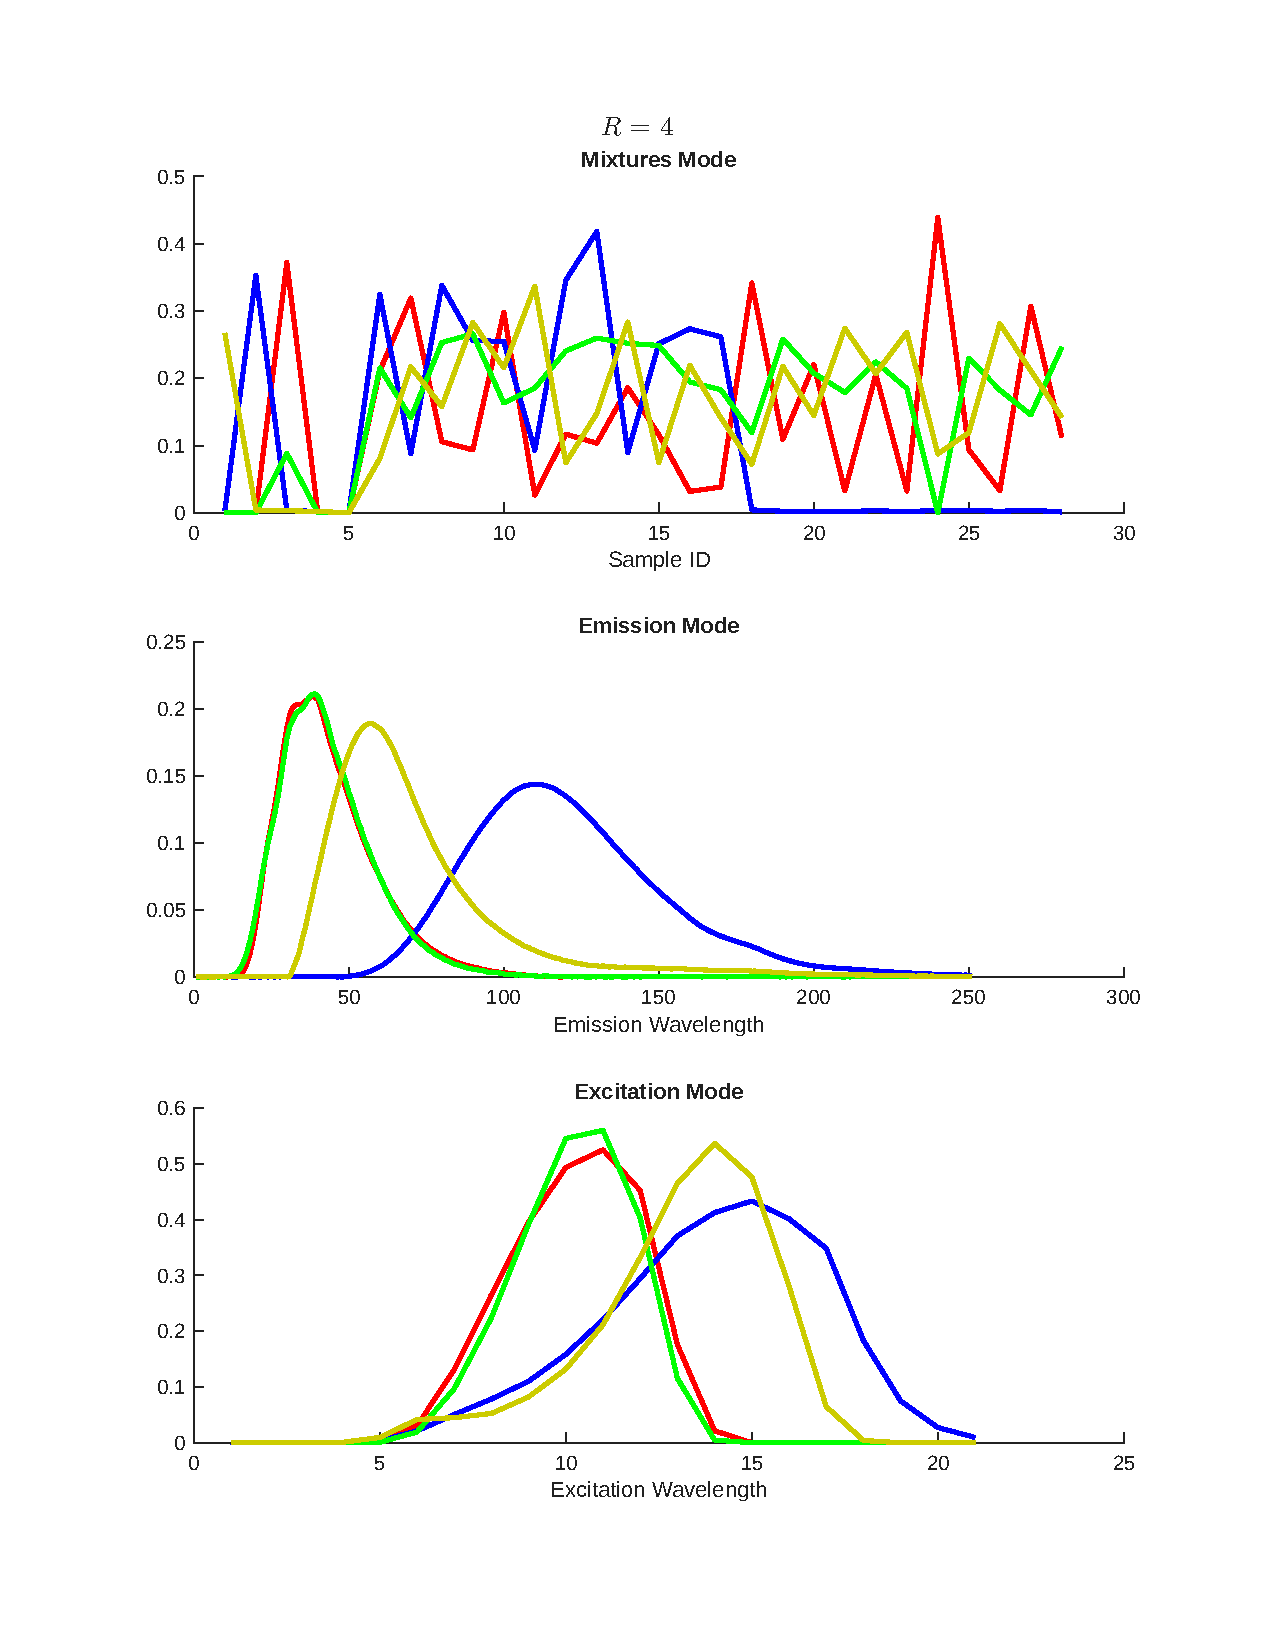
\includegraphics[trim = 2cm 2.5cm 2cm 1.9cm, clip, width=0.46\linewidth]{figures/factors_rank4.pdf}
    \caption{Plots of normalized factors for each mode from the best CP-model over 20 runs for $R=3$ (left) and $R=4$.}
    \label{fig:plot_factors}
\end{figure}

Lastly, we plotted the factors in each mode for the best model for $R=3$ and $R=4$, as seen in Figure \ref{fig:plot_factors}.
We plotted $R=4$ only to confirm our choice of $R$, as discussed above.
For the $R=3$ plots, we see that the model seems to have discovered three different chemicals.
The top left plot, the mixtures mode, represents the amount of each chemical in each of the 28 mixtures, while the plots below represent emission and excitation wavelengths for each chemical.
It is expected that the top plot is less smooth than the two below, as there is no reason why the amount of each chemical in each mix should be a smooth function.
For the wavelengths however, it is expected that the plot for each chemical is quite smooth.
